\documentclass[a4paper,11pt]{article}

\usepackage[slovene]{babel}
\usepackage[T1]{fontenc}
\usepackage[utf8]{inputenc}
\usepackage{lmodern}

\usepackage{textcase}
\usepackage{amsmath}
\usepackage{amsfonts}
\usepackage{amsthm}
\usepackage{fancyhdr}
\usepackage[italicdiff]{physics}
\usepackage{url}
\usepackage{graphicx}

\graphicspath{ {./images/}}

\pagestyle{fancy}
\fancyhf{}
\rhead{\thepage}
\lhead{\textsc{\textsc{Seminarska naloga iz statistike}}}

\setlength{\parskip}{1em}

\newcommand{\ols}[1]{\mskip.5\thinmuskip\overline{\mskip-.5\thinmuskip {#1} \mskip-.5\thinmuskip}\mskip.5\thinmuskip} % overline short
\newcommand{\olsi}[1]{\,\overline{\!{#1}}} % overline short italic

\newcommand{\sumin}{\sum_{i = 1}^n}
\newcommand{\sumiN}{\sum_{i = 1}^N}

\newcommand{\inv}{^{-1}}

\AtBeginDocument{
    \renewcommand{\var}[1]{\operatorname{var}(#1)}
}
    
\DeclareMathOperator{\se}{se}
\DeclareMathOperator{\bin}{Bin}

%%%%%%%%%%%%%%%%%%%%%%%%%%%%%%%%%%%%%%%%%%%%%%%%%%%%%%%%%%%%%%%%

\begin{document}
    
\author{\textbf{Izak Jenko}}
\title{SEMINARSKA NALOGA IZ STATISTIKE}
\date{20. avgust 2021}

\maketitle
\thispagestyle{empty}

\par
Seminarska naloga iz statistike pri predmetu statistika na Fakulteti za matematiko in fiziko v Ljubljani v študijskem letu 2020/21. Celoten repozitorij seminarske naloge, ki vključuje skripte in izračune, najdemo na naslovu:
\begin{center}
    \url{https://github.com/kazi99/STAT-seminarska} 
\end{center}

\section*{1. naloga}

Naj $x_i$ označuje dohodek $i$-te družine za $1 \leq i \leq N := 43 886$. Vzamemo enostavni slučajni vzorec $X_i := x_{K_i}$, kjer je slučajni vektor $(K_1, \ldots, K_n)$ enakomerno porazdeljen po množici $n$-teric s samimi različnimi komponentami, ki prihajajo iz množice $\{ 1, \dots, N\}$. Vzorec bo velikosti $n = 400$ in bo \emph{proporcionalno alociran}, da bomo lahko na koncu primerjali točki a) in b).

\noindent
\textbf{a)} Populacijsko povprečje $\mu = \frac1N \sum_{i=1}^N x_i$ točkovno ocenimo z vzorčnim povprečjem
\[
    \olsi{X} = \frac1n \sum_{i = 1}^n X_i,  
\]
ki na našem vzorcu znaša $43410.49$. Označimo s $\sigma^2 = \frac{1}{N}\sum_{i = 1}^N (x_i - \mu)^2$ populacijsko varianco. Varianca cenilke $\olsi{X}$ bo 
\[
    \var{\olsi{X}} = \frac{\sigma^2}{n}\left(1 - \frac{n-1}{N-1}\right),
\]
kjer faktor $1 - \frac{n-1}{N-1}$ nastopi zaradi koreliranosti posameznih enot enostavnega slučajnega vzorca. Standardna napaka cenilke $\olsi{X}$, bo torej $\se = \frac{\sigma}{\sqrt{n}} \sqrt{1 - \frac{n-1}{N-1}}$. Popoulacijske variance $\sigma^2$ običajno ne poznamo, je pa 
\[
    s^2 = \frac{1}{n-1}\sumin(X_i - \olsi{X})^2, 
\]
njena nepristranska cenilka, torej standardno napako ($\se$) lahko ocenimo z
\[
    \hat{\se} = \frac{s}{\sqrt{n}}\sqrt{1 - \frac{n}{N}}.
\]
Izračunana na našem vzorcu je ocena standardne napake enaka $1758.62$.

Sedaj imamo zbrane vse podatke, da postavimo $95\%$ interval zaupanja. Stopnja tveganja bo $\alpha = 0.05$, kar pomeni, da bo s priblično takšno verjetnostjo interval zaupanja zgrešil dejansko populacijsko statistiko, ki jo ocenjujemo. Ker imamo opravka z veliko ($400$ -- velikost vzorca) enako porazdeljenimi (porazdelitev je empirična) slučajnimi spremenljivkami, lahko zaradi centralnega limitnega izreka predpostavljamo, da je vzorčno povprečje $\olsi{X}$ porazdeljeno približno normalno. Opomnimo še, da te slučajne spremenljivke niso nujno neodvisne, je pa njihova koreliranost razmeroma majhna pri tako veliki populaciji kot je naša, zato je uporaba izreka nekoliko bolj utemeljena. 

Držimo se standardnih oznak in označimo s $\Phi$ kumulativno porazdelitveno funkcijo standardne normalne porazdelitve
\[
    \Phi(x) = \frac{1}{\sqrt{2 \pi}} \int_{-\infty}^{x} e^{-z^2/2}dz.
\]
Če bi poznali populacijsko varianco $\sigma^2$ in s tem standardno napako, bi dobili inteval zaupanja   
\begin{equation}
    \label{normalni IZ}    
    \left(\olsi{X} - \se \Phi\inv\left(1 - \frac{\alpha}{2}\right), 
    \olsi{X} + \se \Phi\inv\left(1 - \frac{\alpha}{2}\right)\right).
\end{equation}
Kar pri našem vzorcu pride $\left( 39963.65, 46857.32\right)$ in je dolžine $6250.57$.

Glede na to pa, da imamo tudi oceno standardne napake in recimo prave vrednosti standardne napake ne bi poznali, lahko postavimo tudi aproksimativni interval zaupanja oblike
\begin{equation}
    \label{aproksimativni IZ}
    \left(\olsi{X} - \hat{\se} \Phi\inv\left(1 - \frac{\alpha}{2}\right), 
    \olsi{X} + \hat{\se} \Phi\inv\left(1 - \frac{\alpha}{2}\right)\right).
\end{equation}
ki je asimptotično eksakten. Na našem vzorcu znaša $\left( 35937.86, 41475.80\right)$ in je dolžine $5537.94$. 
V tem primeru, ko poznamo samo oceno standardne napake, si lahko pomagamo tudi s Studentovo $t$-porazdelitvijo in tako dobimo Studentov interval zaupanja
\begin{equation}
    \label{studentov IZ}
    \left(\olsi{X} - \hat{\se} F_{\text{Student}(n-1)}\inv\left(1 - \frac{\alpha}{2}\right), 
    \olsi{X} + \hat{\se} F_{\text{Student}(n-1)}\inv\left(1 - \frac{\alpha}{2}\right)\right),
\end{equation}
kjer $F_{\text{Student}(n-1)}$ označuje kumulativno porazdelitveno funkcijo Studentove $t$-porazdelitve z $n-1$ prostostnimi stopnjami. Na našem vzorcu pride interval zaupanja $\left(35929.43, 41484.23\right)$, ki je dolžine $5554.79$.

\noindent
\textbf{b)} V tej točki si bomo pogledali kako dobro lahko ocenimo statistike od prej, če si pomagamo s stratificiranjem prebivalstva po četrtih. Naš vzorec velkosti $400$ je stratifician s proporcionalno alokacijo, kar pomeni, da vzamemo $n_1 = 92$ enot iz severne četrti, $n_2 = 95$ iz vzhodne, $n_3 = 123$ iz južne in $n_4 = 90$ iz zahodne četrti kot kaže tabela.
\begin{center}
\begin{tabular}{|c || c c c c ||}
    \hline
    & Sever & Vzhod & Jug & Zahod \\
    \hline
    $n_j$ & $92$ & $95$ & $123$ & $90$ \\
    \hline 
\end{tabular}
\end{center}
Do teh števil pridemo, tako da nekoliko prilagodimo količine $n_j \approx n \cdot w_j$ (tu je $w_j$ delež populacije, ki živi v $j$-ti četri). Polovico od količin $n_j$ zaokrožimo navzgor do najbližjega celega števila, preostale pa navzdol do celega števila.

Najprej stratumsko ocenimo populacijsko povprečje $\mu$ kot
\[
    \olsi{X}_s = \sum_{j = 1}^4 w_j \olsi{X}_j, \quad \text{ kjer je } \quad \olsi{X}_j = \frac{1}{n_j}\sum_{i = 1}^{n_j} X_{ij}
\]
Stratificirana standardna napaka se izraža kot
\[
    \se^2_s = \sum_{j = 1}^4 \frac{w_j^2 \sigma_j^2}{n_j}\left(1 - \frac{n_j - 1}{N_j - 1}\right), 
\]
kjer je stratificirana populacijska varianca $\sigma_j^2 = \sum_{i = 1}^{n_j} \frac{(X_{ij} - \mu_j)^2}{N_j}$. 

Ocena standardne napake bo tedaj 
\[
    \hat{se}^2_s = \sum_{j = 1}^4 \frac{w_j^2 \hat{\sigma}_j^2}{n_j}\left(1 - \frac{n_j - 1}{N_j - 1}\right),
\] 
kjer je $\hat{\sigma}^2_j = \sum_{i = 1}^{n_j} \frac{(X_{ij} - \olsi{X}_j)^2}{n_j - 1}$ nepristranska cenilka populacijske variance v $j$-tem stratumu $\sigma_j^2$.

Sedaj lahko podobno kot prej postavimo $95\%$ intervale zaupanja. Najprej če predpostavjlamo, da poznamo populacijsko varianco, dobimo
\[
    \left(\olsi{X}_s - \se_s \cdot \Phi\inv\left(1 - \frac{\alpha}{2}\right), 
    \olsi{X} + \se_s \cdot \Phi\inv\left(1 - \frac{\alpha}{2}\right)\right).
\] 
Na našem vzorcu je to $\left(36604.38, 42106.27\right)$, ki je dolžine $6224.06$, kar pomeni, da je krajši kot interval \eqref{normalni IZ} in s tem tudi boljši za ocenejevanje povprečnega dohodka. 

Naslednji je aproksimativni interval zaupanja, kjer uporabimo oceno za standardno napako $\hat{\se}_s$. Interval bo tedaj 
\[
    \left(\olsi{X}_s - \hat{\se}_s \cdot \Phi\inv\left(1 - \frac{\alpha}{2}\right), 
    \olsi{X} + \hat{\se}_s \cdot \Phi\inv\left(1 - \frac{\alpha}{2}\right)\right), 
\]
ki bo pri naših podatkih $\left(35931.97, 41480.80\right)$ dolžine $5548.84$, kar je pravtako krajše kot interval \eqref{aproksimativni IZ} in tako boljše kot če ne bi stratificirali.

Nazadnje lahko postavimo še Studentov interval zaupanja za ocenejevanje povprečja, pred tem pa moramo izračunati prostostne stopnje
\[
    \hat{\nu} = \frac{\hat{\se}^2_s}{\sum_{j = 1}^4 \frac{w_j^4 \hat{\sigma}^2_j}{n_j^2 (n_j - 1)}}.  
\]
Interval zaupanja bo tako oblike
\[
    \left(\olsi{X} - \hat{\se} \cdot F_{\text{Student}(\hat{\nu})}\inv\left(1 - \frac{\alpha}{2}\right), 
    \olsi{X} + \hat{\se} \cdot F_{\text{Student}(\hat{\nu})}\inv\left(1 - \frac{\alpha}{2}\right)\right),  
\]
na naših podatkih bo to interval $\left(35931.97, 41480.80\right)$ dolžine $5548.84$, ki je spet boljši kot \eqref{studentov IZ}, ko nismo stratificirali.

Intervale zaupanja prikažemo tudi grafično.
\begin{center}
    \begin{figure}[h]
        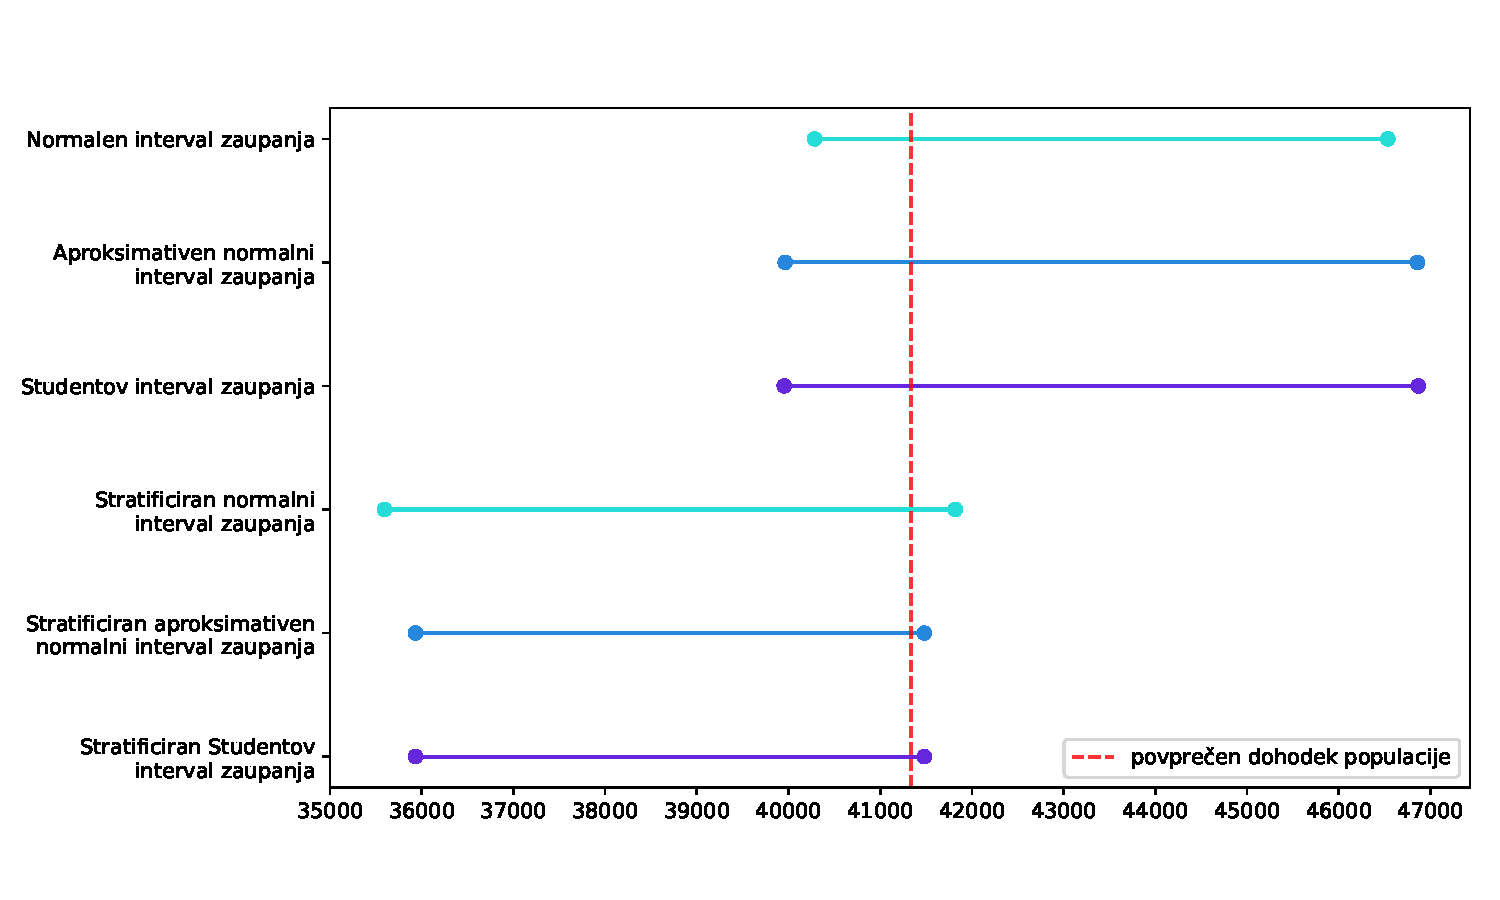
\includegraphics[scale=0.5]{intervali_zaupanja}
        \caption{$95\%$ intervali zaupanja}
    \end{figure}
\end{center}
Zaključimo lahko, da je v tem primeru bilo bolj ugodno stratificirati po četrtih, saj smo tako dobili ožje intevale zaupanja, kar nam bo omogočilo postaviti bolj natančne ocene povprečnega dohodka v Kibergradu. 

Do računskih razultatov pri tej nalogi smo prišli s pomočjo priloženih skript \texttt{naloga\_1a.ipynb} in \texttt{naloga\_1b.ipynb}, ki analizirata isti enostaven slučajni vzorec $400$ enot (s proporcionalno alokacijo) iz datoteke \texttt{vzorec.csv}.

\section*{2. naloga}

Imamo vzorec $280$ palic, kjer smo vsaki od njih preizkusili lomljivost na petih mestih. Sumimo, da je število mest na katerih se je palica zlomila porazdeljeno $\bin(5,p)$, kar bo tudi naša osnovna ničelna domneva $H_0$.

\noindent
\textbf{a)} Denimo, da osnovna ničelna domneva velja, po metodi največjega verjetja pa ocenimo parameter $p$. Vzemimo
\[
    L_1(p; x) = \mathsf{P}_p(X = x) = \binom{5}{x}p^x(1-p)^{5 - x},
\]
kjer je slučajna spremenljivka $X$ porazdeljena binomsko $\bin(5,p)$. Verjetje bo tedaj funkcija
\[
    L(p; x_1, \ldots, x_n) = \prod_{i = 1}^n L_1(p; x) = \prod_{i = 1}^n \binom{5}{x_i}p^x_i(1-p)^{5 - x_i}.
\]
Cenilka za $p$ bo torej tisti parameter, pri katerem je verjetje maksimalno. Ker je verjertje gladko odvisno od parametra $p \in (0,1)$ bomo ta ekstrem poiskali z odvodom, da bo računanje lažje pa si bomo pomagali z logaritmom verjetja
\begin{multline*}
    \ell(p; x_1, \ldots, x_n) := 
    \log L(p; x_1, \ldots, x_n) \\ 
    = \sumin \log\binom{5}{x_i} + \sumin x_i\log(p) + \sumin(5 - x_i) \log(5 - p)
\end{multline*}
Z odvajanjem $\ell$ po $p$ dobimo
\[
    \ell'(p; x_1, \ldots, x_n) =
    \sumin \left( \frac{x_i}{p} - \frac{5 - x_i}{1 - p}\right) = 
    \sumin \frac{x_i - 5p}{p - p^2}.
\]
Ta odvod bo enak $0$ natanko tedaj, ko bo $p = \frac{1}{5n} \sumin x_i$, torej cenilko za $p$ vzamemo 
\[
    \hat{p} = \frac{\olsi{X}}{5}, \quad \text{ kjer je $\olsi{X}$ vzorčno povprečje.}  
\] 


\begin{thebibliography}{99}

    \bibitem{Rice}
    J.~Rice, \emph{Mathematical statistics \& data analysis}, third edition, Duxbury, 2007
    
\end{thebibliography}

\end{document}